\documentclass[10pt, conference]{IEEEtran}

\usepackage{cite}
\usepackage{amsmath,amssymb,amsfonts}
\usepackage{graphicx}
\usepackage{textcomp}
\usepackage{xcolor}
\usepackage{booktabs}
\usepackage{array}
\usepackage{tabularx}
\usepackage{hyperref}
\usepackage{tikz}
\usetikzlibrary{positioning}

\begin{document}

\title{Confidence- and Link-Aware Task Routing for Resilient Maritime Edge AI}

\author{%
\IEEEauthorblockN{Anthony Uchenna Eneh\IEEEauthorrefmark{1}, Love Allen Chijioke Ahakonye\IEEEauthorrefmark{2}, Jae-Min Lee\IEEEauthorrefmark{1}, Dong-Seong Kim\IEEEauthorrefmark{3}}
\IEEEauthorblockA{\IEEEauthorrefmark{1}IT Convergence Engineering, Kumoh National Institute of Technology, Gumi, South Korea}
\IEEEauthorblockA{\IEEEauthorrefmark{2}ICT Convergence Research Center, Kumoh National Institute of Technology, Gumi, South Korea}
\IEEEauthorblockA{\IEEEauthorrefmark{3}IT Convergence Engineering \& NSLab Co., Ltd., Kumoh National Institute of Technology, Gumi, South Korea}
}
\maketitle

\begin{abstract}
Mobile and maritime systems increasingly depend on edge AI for situational awareness, vessel detection, anomaly monitoring, and local operational decisions. These deployments, however, combine intermittent connectivity, constrained compute, heterogeneous link quality, and input shift, making naive local inference or fixed offloading policies brittle. This paper proposes an uncertainty-aware task routing layer for edge AI workloads. For each task, the router chooses among local inference, peer or relay forwarding, and a conservative fallback mode by jointly considering model confidence, queue pressure, urgency, and link state. We evaluate the design using Kaggle's Ships in Satellite Imagery dataset, training a ResNet-18 vessel classifier and deriving confidence traces from nominal and synthetically degraded satellite image chips. In a 37,500-task routing emulation, the three-way router reduces unsafe outcomes under degraded connectivity from 7.3\% for always-local execution and 6.8\% for always-offload execution to 4.8\%, while using fallback for 7.6\% of tasks. Under intermittent connectivity, it reduces unsafe outcomes relative to always-local and confidence-threshold policies, but the experiment also reveals an important limitation: max-softmax confidence remains high for some adverse-condition errors. The results support fallback as a first-class routing action while showing that maritime edge AI still needs stronger calibration or shift detection.
\end{abstract}

\begin{IEEEkeywords}
Edge AI, uncertainty estimation, task routing, maritime IoT, mobile networks, resilient systems.
\end{IEEEkeywords}

\section{Introduction}
Mobile and maritime platforms increasingly depend on edge AI for rapid decisions in the field: vessel sensor anomaly detection, onboard video triage, equipment health monitoring, traffic awareness, and inspection support in disconnected environments. These settings are difficult for standard cloud-centric machine-learning pipelines because links are intermittent, compute budgets are small, and decision latency can be operationally critical~\cite{shi2016edge,satyanarayanan2017emergence}.

This paper studies a simple but useful question: when should an edge node execute AI locally, when should it offload the task to another node, and when should it avoid an uncertain decision and fall back to a conservative policy? The answer matters in mobile and maritime systems because the cost of a wrong decision (e.g., missed collision alert) can be orders of magnitude higher than the cost of a delayed one.

The usual edge-computing framing emphasizes latency reduction, bandwidth savings, and energy efficiency. Those objectives remain important, but they are incomplete for mission-facing mobile systems. A vessel, unmanned surface vehicle, port-side gateway, or field inspection device may be forced to act while satellite backhaul is congested, a relay is temporarily unavailable, or a local model encounters inputs that differ from its training distribution. In such cases, the system needs a routing decision coupled to both prediction confidence and communication state. A policy that always chooses the fastest path may amplify incorrect predictions, while a policy that always offloads may fail exactly when the network is most degraded.

We therefore treat task routing as a runtime control problem with three possible outcomes. The node can use its local model, forward the task to another node with better resources or connectivity, or invoke a safe fallback routine. The fallback option is not intended to outperform the AI model; it is designed to be conservative, explainable, and available under degraded conditions. Examples include threshold rules for equipment alerts, rate-limited human notification, and preserving a prior operational state until stronger evidence arrives.

Our core idea is an uncertainty-aware routing layer that sits above the inference model and below actuation. It uses confidence, queue pressure, urgency, and link quality to choose among local execution, forwarding to a peer or relay node, and fallback to a safe mode. The design is intentionally lightweight so it can fit constrained edge devices. It can consume uncertainty signals from calibration and out-of-distribution detection methods without requiring a new model architecture~\cite{guo2017calibration,hendrycks2017baseline,zhang2022edgeuncertainty}.

Unlike prior uncertainty-aware offloading work that focuses on binary decisions (local vs. offload), this paper introduces a third action---conservative fallback---as a first-class decision rather than a failure mode. This distinction is critical in safety-constrained maritime environments where ``no decision'' is sometimes better than a wrong decision.

\textbf{Contributions.} This short paper makes three contributions:
\begin{itemize}
    \item a compact uncertainty-aware task routing policy for edge AI in mobile and maritime networks;
    \item a deployable systems architecture that separates inference, routing, forwarding, and fallback behavior;
    \item an experimental evaluation showing how fallback-aware routing changes latency, energy, and unsafe execution rates under stable, intermittent, and degraded links.
\end{itemize}

\section{Related Work}
This paper sits at the intersection of edge AI, resilient communications, and mission-critical systems. Prior work on maritime IoT and mobile edge computing shows the need for low-latency local intelligence, while research on uncertainty estimation highlights that not every AI prediction should be trusted equally. Our focus is narrower: a lightweight routing layer that turns uncertainty into an operational decision.

Recent maritime MEC studies provide useful context for routing and offloading design. Bandit-based server selection, distributed optimization, UAV- or AAV-assisted edge computing, and multi-agent reinforcement learning have been used for latency-energy trade-offs and hybrid offloading~\cite{yang2022mab_maritime,you2025joint_maritime,he2025distributed_maritime,kong2025satd3_maritime,ning2025marho}. Fault-tolerant formulations further motivate resilient policies that can maintain service under failures and link degradation~\cite{zhang2024fault_tolerant_edge}.

Compared with this literature, the proposed design is deliberately modest. It does not attempt to solve full resource allocation, multi-agent learning, or optimal placement. Instead, it addresses the local decision that remains when those larger mechanisms are unavailable, too expensive, or not trusted in the field. This makes it complementary to optimization-based MEC approaches: a learned offloading controller may select the best peer under normal operation, while the uncertainty-aware fallback layer can guard against unsafe local execution and broken forwarding paths.

Uncertainty estimation is also relevant. Calibration methods improve the relationship between predicted confidence and empirical correctness~\cite{guo2017calibration}, while out-of-distribution detection methods provide signals that a model may be operating outside its reliable domain~\cite{hendrycks2017baseline}. Recent uncertainty-aware edge-intelligence work broadens this concern to deployment settings where model quality, communication, and resource constraints interact~\cite{zhang2022edgeuncertainty,wang2023adaptiveoffload}. In this paper, uncertainty signals are not treated as final answers. They are transformed into routing constraints and fallback triggers, which is the practical systems role needed in mobile and maritime deployments.

\section{System Methodology}
\subsection{Problem Setting}
We consider a distributed edge system deployed on a mobile or maritime platform, where sensor streams and local AI tasks arrive continuously. Each task has an estimated confidence score and an operational urgency level. For each arrival, the node must decide whether to process the task locally, forward it, or defer to a conservative fallback policy.

The setting differs from ordinary cloud inference in three ways. First, connectivity is unstable, so routing decisions must work even when the network is partially unavailable. Second, the edge node may operate under tight compute and power constraints. Third, the system must preserve operational continuity, meaning that an uncertain AI decision should not silently fail.

We assume a small set of peer nodes or relay nodes may be reachable when links are available. The system must therefore make routing decisions online, with only local state and lightweight network feedback. This is particularly relevant for maritime IoT deployments, which often operate under harsh connectivity constraints~\cite{li2019maritimeiot}.

Let each incoming task be represented as $x_i=(d_i,g_i,s_i)$, where $d_i$ is the sensor payload or feature vector, $g_i$ is the urgency class, and $s_i$ is optional platform state. The local model produces a prediction $\hat{y}_i$ and a confidence estimate $c_i\in[0,1]$. The node also observes a normalized queue load $\bar{q}_i$, a link-quality estimate $\ell_i\in[0,1]$, and a peer availability indicator $a_i$. The action space is
\begin{equation}
    r_i \in \{\text{local}, \text{forward}, \text{fallback}\}.
\end{equation}
The routing objective is deployment-dependent. In a safety-sensitive alerting task, avoiding low-confidence local decisions may dominate latency. In routine monitoring, latency and energy may be weighted more heavily. This motivates a policy that exposes simple thresholds and guardrails rather than hiding the decision entirely inside an opaque optimizer.

The main assumptions are modest. Each node can compute or receive a confidence proxy, maintain approximate queue and link-quality state from local telemetry, and access an application-defined fallback routine. The proposed routing layer does not invent the safe action; it decides when the safe action should be preferred.

\noindent\textbf{Objective.} Let the cost of handling task $i$ under action $r_i$ be:
\begin{equation}
    C(r_i) = w_1 \cdot \ell(r_i) + w_2 \cdot e(r_i) + w_3 \cdot \mathbf{1}_{\text{unsafe}}(r_i) \cdot \Delta_{\text{safety}}
\end{equation}
where $\ell(r_i)$ is latency, $e(r_i)$ is energy consumption, $\mathbf{1}_{\text{unsafe}}(r_i)=1$ if the action leads to a wrong high-impact decision (e.g., missed collision alert or false emergency), and $\Delta_{\text{safety}}$ is the safety penalty. The routing policy aims to minimize expected cost $\mathbb{E}[C(r_i)]$ given uncertain observations of connectivity, resource state, and model confidence. This formulation makes explicit why a conservative fallback may be optimal: it avoids the large safety penalty $\Delta_{\text{safety}}$ when confidence is low and connectivity is poor.

\subsection{System Architecture}
Figure~\ref{fig:arch} sketches the system. Sensor tasks enter a lightweight preprocessing stage, after which the local model and uncertainty estimator produce a candidate prediction. The routing policy then chooses among local completion, peer forwarding, or fallback. The output of the router is logged with enough metadata to support later auditing: confidence bucket, link state bucket, selected action, and completion status.

\begin{figure}[t]
\centering
\resizebox{\columnwidth}{!}{%
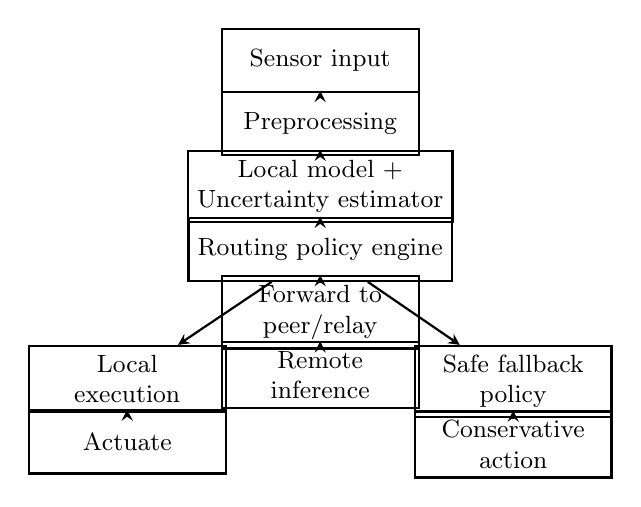
\begin{tikzpicture}[
    node distance=0.8cm,
    block/.style={rectangle, draw, thick, minimum width=2.5cm, minimum height=0.8cm, align=center, font=\small},
    arrow/.style={-stealth, thick}
]
\node[block] (sensor) {Sensor input};
\node[block, below of=sensor] (preprocess) {Preprocessing};
\node[block, below of=preprocess] (model) {Local model +\\Uncertainty estimator};
\node[block, below of=model] (router) {Routing policy engine};
\node[block, below left=0.8cm and -0.5cm of router] (local) {Local\\execution};
\node[block, below of=router] (forward) {Forward to\\peer/relay};
\node[block, below right=0.8cm and -0.5cm of router] (fallback) {Safe fallback\\policy};
\node[block, below of=local] (actuate) {Actuate};
\node[block, below of=forward] (remote) {Remote\\inference};
\node[block, below of=fallback] (safe) {Conservative\\action};

\draw[arrow] (sensor) -- (preprocess);
\draw[arrow] (preprocess) -- (model);
\draw[arrow] (model) -- (router);
\draw[arrow] (router) -- (local);
\draw[arrow] (router) -- (forward);
\draw[arrow] (router) -- (fallback);
\draw[arrow] (local) -- (actuate);
\draw[arrow] (forward) -- (remote);
\draw[arrow] (fallback) -- (safe);
\end{tikzpicture}%
}
\caption{System architecture: sensor input flows through preprocessing, local inference, and uncertainty estimation before the routing policy chooses among local execution, peer forwarding, or safe fallback.}
\label{fig:arch}
\end{figure}

The router is intentionally placed after model scoring but before external actuation. This placement lets the node use model uncertainty without changing the model itself. It also keeps application-specific fallback logic separate from the learned model. For example, an onboard anomaly detector can still run as usual, but alerts below a confidence threshold may be converted into a low-priority inspection request instead of triggering an immediate automated response.

The forwarding path is opportunistic rather than mandatory. A node may forward a task to a better-connected relay, a nearby gateway, or a peer with a stronger accelerator. If no acknowledgment is received within a bounded time, the task returns to the router and is either executed locally or sent to fallback depending on urgency and confidence. This prevents indefinite waiting on broken links.

The architecture also supports auditability. Each decision can be logged as a compact tuple containing confidence bucket, urgency class, queue bucket, link bucket, selected action, and completion status. These logs help operators tune thresholds after deployment and explain why a task was not handled by the learned model.

\subsection{Routing Policy}
Our method is a three-way policy:
\begin{itemize}
    \item \textbf{Local execution:} run inference on the current edge node when confidence is high and the queue is manageable.
    \item \textbf{Forwarding:} offload the task to a peer or relay node when local load is high but network quality is acceptable.
    \item \textbf{Fallback:} use a safe rule-based mode when confidence is low or the network is too degraded for reliable offload.
\end{itemize}

The routing score combines normalized signals for confidence, queue pressure, link quality, and urgency. We define uncertainty as $z_i=1-c_i$. A simple deployable score for local execution is
\begin{equation}
    S_{local}=\alpha c_i - \beta \bar{q}_i + \gamma \kappa_i,
\end{equation}
where $\kappa_i$ captures urgency-dependent preference for immediate local action. A forwarding score is
\begin{equation}
    S_{forward}=\lambda \ell_i + \mu \bar{q}_i - \nu z_i,
\end{equation}
which favors forwarding when the local queue is pressured, the link is usable, and the model is not too uncertain. A fallback score is
\begin{equation}
    S_{fallback}=\rho z_i + \eta (1-\ell_i) + \delta \phi_i,
\end{equation}
where $\phi_i$ indicates whether the task belongs to a safety-sensitive class.

The chosen action is the maximum-score action subject to guardrails. In particular, forwarding is disallowed when $a_i=0$ or $\ell_i$ is below a minimum threshold, and local execution is disallowed for safety-sensitive tasks whose confidence is below a configured floor. These guardrails are important because they express operational requirements that should not be learned away by a throughput-oriented policy.

In practice, this can be implemented with a small threshold-based controller or a learned policy. This paper focuses on the threshold-based version because it is easier to deploy, inspect, and certify. Related maritime MEC offloading work typically optimizes latency and energy through bandit, distributed optimization, and multi-agent reinforcement learning formulations~\cite{shi2020edgeai,yang2022mab_maritime,he2025distributed_maritime,ning2025marho}, while our emphasis is on operational safety under uncertainty rather than pure throughput maximization.

The policy can be tuned in two stages. Offline, historical traces or simulated traces are used to choose conservative starting thresholds. Online, the node updates moving averages for queue delay and link quality, but it does not need to retrain the AI model. This separation is useful for maritime deployments where field updates are costly and operators may require predictable behavior before accepting autonomous routing changes.

\subsection{Failure Handling}
Edge AI systems fail in several different ways, and the routing layer should distinguish them. A low-confidence prediction is not the same as a saturated queue, and a weak link is not the same as a peer failure. Treating these cases separately makes the system easier to diagnose and safer to operate.

\noindent\textbf{Concrete fallback examples.} The meaning of ``conservative fallback'' depends on the application. Table~\ref{tab:fallback_examples} provides maritime-specific illustrations.

\begin{table}[t]
\centering
\caption{Maritime fallback examples by application domain}
\label{tab:fallback_examples}
\footnotesize
\setlength{\tabcolsep}{3pt}
\begin{tabularx}{\columnwidth}{@{}>{\raggedright\arraybackslash}p{0.28\columnwidth}>{\raggedright\arraybackslash}p{0.32\columnwidth}>{\raggedright\arraybackslash}X@{}}
\toprule
\textbf{Application} & \textbf{Full inference (local/offload)} & \textbf{Fallback action} \\
\midrule
Vessel collision avoidance & Predict intent (e.g., crossing, overtaking) of nearby vessel & Reduce speed, sound horn, maintain heading, alert operator \\
Maritime surveillance & Classify ship/no-ship satellite image chip & Flag chip for review, defer alert, request another pass \\
Engine anomaly detection & Classify fault type from vibration spectrogram & Report ``inspection needed'', log raw data, use limit-based alert \\
Navigation waypoint decision & Select optimal path from camera/LiDAR & Hold position, revert to last safe heading, request human review \\
Cargo monitoring & Predict temperature anomaly from sensor fusion & Use last valid reading $+$ conservative drift bound, flag uncertainty \\
\midrule
\end{tabularx}
\end{table}

For connectivity degradation, the router uses bounded retries and timeouts. A forwarded task is marked pending only for a short interval determined by urgency. When the timeout expires, the router recomputes the action using the current state. For compute pressure, the node raises the load term and may prefer forwarding if links are healthy. For model uncertainty, the router avoids forwarding tasks that are already outside the model's reliable region unless a remote node has a known stronger model, broader context, or fresher calibration.

Fallback behavior should be conservative and auditable. For anomaly detection, fallback may report an ``inspection required'' state rather than a binary fault decision. For navigation awareness, fallback may preserve the last safe recommendation and request additional sensing. For equipment monitoring, fallback may trigger a rule based on physical limits rather than learned features. The common requirement is that fallback should make uncertainty visible instead of hiding it behind a confident but unreliable prediction.

The router also needs a fail-closed mode. If both local confidence and network state are poor for a safety-sensitive task, the correct behavior is not to force an AI decision. Instead, the task should be converted into a safe operational state, deferred for human review, or logged as unresolved depending on the application.

\section{Experimental Evaluation}
We implemented the routing policy in a compact Python emulation to answer three questions: (i) whether uncertainty-aware routing reduces unsafe outcomes, (ii) whether latency remains acceptable under link disruption, and (iii) whether conservative fallback is used selectively rather than as a default response.

\subsection{Experimental Setup}
The experiment uses Kaggle's Ships in Satellite Imagery dataset (ShipsNet)~\cite{shipsnet_kaggle}, which contains 4,000 PlanetScope satellite image chips of size $80\times80$: 1,000 ship images and 3,000 no-ship images. This dataset better matches the paper's maritime monitoring motivation than a generic natural-image benchmark because the inference task is vessel detection in coastal satellite imagery.

We train a binary ResNet-18 classifier initialized from ImageNet weights. The dataset is split into 2,800 training images, 600 validation images, and 600 held-out test images with stratified class balance. After three epochs on CPU, the classifier reaches 84.8\% validation accuracy. We then extract confidence traces from 500 held-out images in two conditions: the original nominal satellite chips and an adverse condition generated by deterministic contrast reduction, brightness reduction, Gaussian blur, haze blending, and sensor-like noise. The adverse transformation is not intended to be a full weather simulator; it is a repeatable stressor for visibility degradation.

Table~\ref{tab:classifier_traces} summarizes the confidence traces. Nominal accuracy is 88.8\%, while adverse-condition accuracy drops to 75.0\%. The mean confidence, however, is higher in the adverse condition. This overconfidence is an important result: simple max-softmax confidence is useful as a routing signal, but it does not fully detect maritime image degradation.

\begin{table}[t]
\centering
\caption{Held-out ShipsNet confidence traces}
\label{tab:classifier_traces}
\footnotesize
\begin{tabular}{@{}lrrrr@{}}
\toprule
\textbf{Condition} & \textbf{Samples} & \textbf{Acc.} & \textbf{Mean Conf.} & \textbf{Std.} \\
\midrule
Nominal & 500 & 88.8\% & 0.810 & 0.140 \\
Adverse & 500 & 75.0\% & 0.842 & 0.085 \\
\bottomrule
\end{tabular}
\end{table}

Each policy is evaluated on 2,500 tasks per network scenario, producing 37,500 task decisions across five policies and three scenarios. The scenarios are:
\begin{itemize}
    \item \textbf{Stable:} 5--12 Mbps bandwidth, 90\% peer availability, 3\% loss, and 20 ms base network latency.
    \item \textbf{Intermittent:} 0.8--6 Mbps bandwidth, 70\% peer availability, 12\% loss, and 40 ms base network latency.
    \item \textbf{Degraded:} 0.2--2.5 Mbps bandwidth, 40\% peer availability, 30\% loss, and 80 ms base network latency.
\end{itemize}

The task stream samples adverse-condition traces with probability 0.4 and marks 30\% of tasks as safety-sensitive. The compared policies are always local, always offload when a peer is available, confidence-threshold offloading, load-only offloading, and the proposed three-way policy. The confidence-threshold policy forwards tasks with confidence below 0.70. The load-only policy forwards when simulated queue pressure exceeds 0.5 and a peer is available. The proposed router uses confidence and bandwidth guardrails: it falls back when confidence is below 0.65 and bandwidth is below 1.8 Mbps, offloads when bandwidth is above 1.8 Mbps and a peer is available, and otherwise executes locally.

Latency and energy are computed with an emulated cost model. Local execution latency increases as confidence decreases. Offloading adds network delay and may fail when a peer is unavailable or packet loss occurs. Fallback has fixed low latency and low energy because it represents a conservative rule-based response rather than neural inference. We define the unsafe rate as the fraction of all tasks that produce an unsafe emulated outcome: a safety-sensitive wrong or low-confidence local decision, or a safety-sensitive offload failure. Thus, the metric captures routing-layer operational risk, not physical maritime incidents.

\begin{figure}[t]
\centering
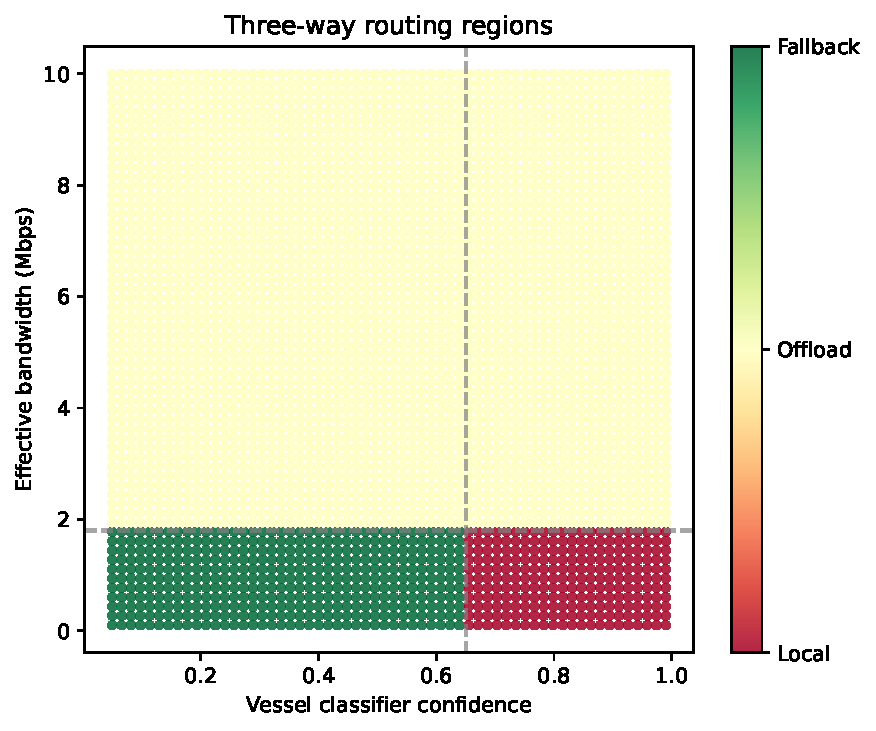
\includegraphics[width=\columnwidth]{figures/decision_boundary.pdf}
\caption{Three-way routing regions for the implemented threshold policy. Fallback is selected only when classifier confidence and bandwidth are both below configured guardrails.}
\label{fig:decision_boundary}
\end{figure}

\subsection{Baseline Comparison}
Table~\ref{tab:main_results} reports the intermittent-connectivity case, which is a representative operating point for mobile and maritime networks. Always-local execution is fastest but ignores confidence and produces a 5.8\% unsafe rate. Always-offload reduces unsafe outcomes to 4.3\%, but increases mean latency to 71.6 ms because it depends on peer availability and link quality. Confidence-threshold offloading lowers unsafe outcomes relative to always-local execution, but still forwards tasks without considering bandwidth. Load-only routing obtains the lowest unsafe rate in this scenario, but at higher latency than the proposed policy.

\begin{table}[t]
\centering
\caption{Performance under intermittent connectivity}
\label{tab:main_results}
\footnotesize
\setlength{\tabcolsep}{3pt}
\resizebox{\columnwidth}{!}{%
\begin{tabular}{@{}lrrrr@{}}
\toprule
\textbf{Policy} & \textbf{Lat.} & \textbf{Unsafe} & \textbf{Energy} & \textbf{Fallback} \\
 & \textbf{(ms)} & \textbf{Rate} & \textbf{(J)} & \textbf{Rate} \\
\midrule
Always Local & \textbf{49.4} & 5.8\% & 0.50 & 0.0\% \\
Always Offload & 71.6 & 4.3\% & 0.59 & 0.0\% \\
Confidence Threshold & 59.6 & 4.9\% & \textbf{0.53} & 0.0\% \\
Load Only & 67.0 & \textbf{3.8\%} & 0.57 & 0.0\% \\
Three-Way (Ours) & 61.6 & 4.4\% & 0.56 & 2.6\% \\
\bottomrule
\end{tabular}
}
\end{table}

The three-way router is not uniformly best in the intermittent case, but it provides a balanced safety-latency trade-off. Compared with always-local execution, unsafe outcomes fall from 5.8\% to 4.4\%, a relative reduction of 24.8\%. Compared with confidence-threshold offloading, unsafe outcomes fall from 4.9\% to 4.4\% while latency increases only modestly relative to local execution. Load-only routing obtains a lower unsafe rate, but its latency is 5.4 ms higher than the three-way policy. This result supports the paper's narrower claim: fallback-aware routing is valuable as a guardrail, especially when link degradation and uncertainty occur together, but it does not replace the need for good calibration and workload-specific threshold tuning.

\subsection{Behavior Across Network Conditions}
Table~\ref{tab:threeway_behavior} shows how the proposed router changes behavior across link conditions. Under stable links, the router uses no fallback and behaves mostly like an offloading policy. Under intermittent links, it uses a mixed strategy: 55.2\% offload, 42.2\% local, and 2.6\% fallback. Under degraded links, fallback rises to 7.6\%, local execution rises to 81.1\%, and offloading drops to 11.3\% because peer availability and bandwidth no longer justify network dependence.

\begin{table}[t]
\centering
\caption{Three-way router behavior across network conditions}
\label{tab:threeway_behavior}
\footnotesize
\setlength{\tabcolsep}{3pt}
\resizebox{\columnwidth}{!}{%
\begin{tabular}{@{}lrrrrrr@{}}
\toprule
\textbf{Scenario} & \textbf{Lat.} & \textbf{Unsafe} & \textbf{Energy} & \textbf{Local} & \textbf{Offload} & \textbf{Fallback} \\
 & \textbf{(ms)} & \textbf{Rate} & \textbf{(J)} & \textbf{Rate} & \textbf{Rate} & \textbf{Rate} \\
\midrule
Stable & 33.5 & 1.5\% & 0.59 & 10.7\% & 89.3\% & 0.0\% \\
Intermittent & 61.6 & 4.4\% & 0.56 & 42.2\% & 55.2\% & 2.6\% \\
Degraded & 58.5 & 4.8\% & 0.50 & 81.1\% & 11.3\% & 7.6\% \\
\bottomrule
\end{tabular}
}
\end{table}

The degraded case is the clearest setting for the proposed policy. Always-offload reaches 98.2 ms latency and a 6.8\% unsafe rate, confidence-threshold offloading reaches 78.9 ms and a 7.0\% unsafe rate, and load-only routing reaches 91.8 ms and a 7.2\% unsafe rate. The proposed router reduces unsafe outcomes to 4.8\% and keeps latency at 58.5 ms by avoiding fragile offload attempts and invoking fallback for a bounded subset of tasks. This behavior is desirable in safety-sensitive maritime systems because poor connectivity should not force the system into either a brittle remote dependency or an untrusted local action.

\begin{figure*}[t]
\centering
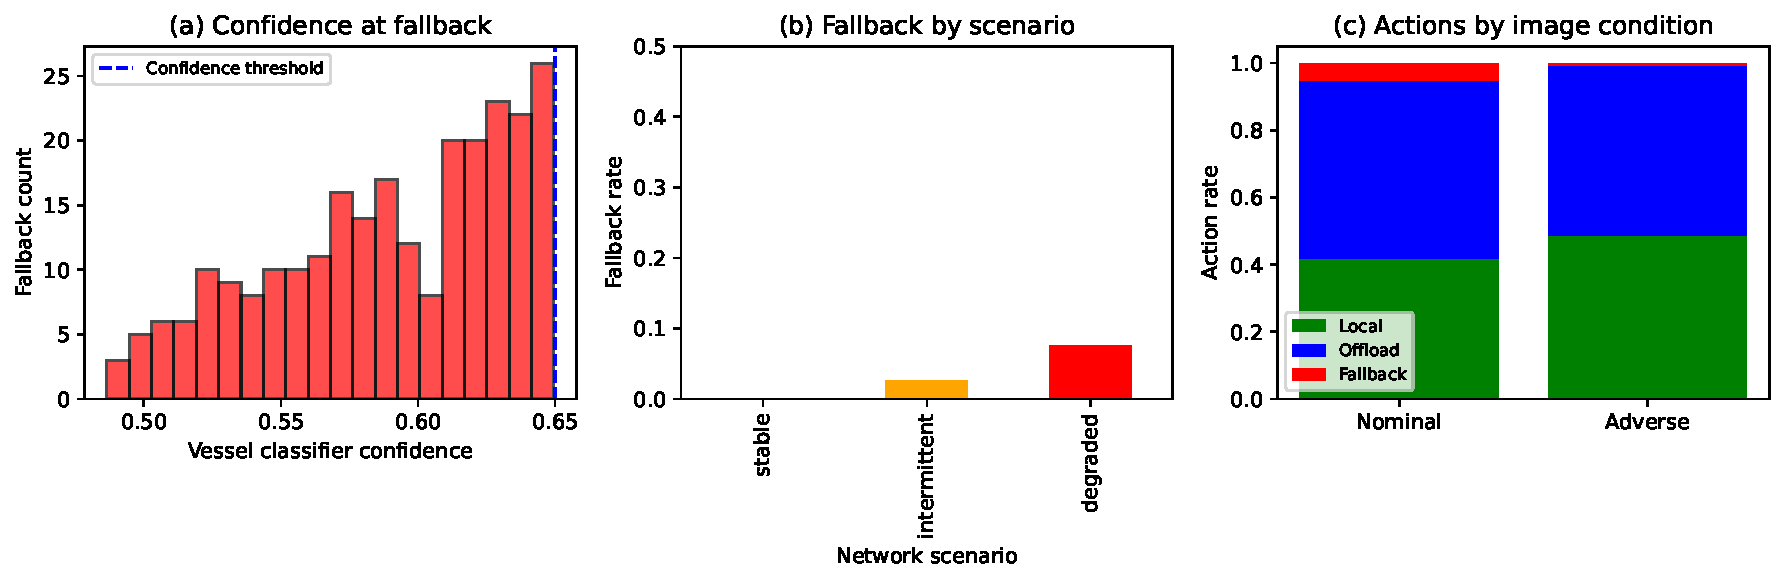
\includegraphics[width=0.95\textwidth]{figures/fallback_analysis.pdf}
\caption{Fallback analysis for the three-way policy on ShipsNet traces: fallback events occur below the confidence threshold, increase as connectivity degrades, and differ between nominal and adverse image conditions.}
\label{fig:fallback_analysis}
\end{figure*}

Figure~\ref{fig:fallback_analysis} further explains fallback behavior. The confidence histogram confirms that fallback is triggered for low-confidence tasks, while the scenario-level plot shows that fallback is primarily a degraded-connectivity response. Across all scenarios for the three-way policy, fallback is 5.2\% for nominal traces and 0.7\% for adverse traces. This counterintuitive result occurs because the classifier is sometimes more confident under the synthetic adverse transformation even when accuracy falls. The finding is useful because it exposes a real deployment concern: confidence-only fallback will miss overconfident shifted inputs unless confidence is calibrated or augmented with explicit shift detection.

Overall, the results support the main design claim: conservative fallback is not merely a recovery mechanism after failure. It is a useful third routing action that lets the system preserve continuity under degraded links, while the overconfidence observed on adverse satellite chips shows why uncertainty quality matters.

\section{Limitations and Future Work}

The proposal has several limitations that point to future research directions.

\noindent\textbf{Calibration dependence.} The router assumes confidence scores are meaningful and calibrated. The ShipsNet experiment shows why this is a serious assumption: adverse image degradation lowers classifier accuracy while mean confidence remains high. Future work should incorporate online calibration~\cite{guo2017calibration}, conformal prediction, or explicit shift/OOD detectors rather than relying only on max-softmax confidence.

\noindent\textbf{Peer capability metadata.} Forwarding assumes the node knows what remote peers can do (e.g., model version, accelerator type, current load). In ad-hoc maritime networks, this requires lightweight service discovery or periodic beaconing, which adds overhead.

\noindent\textbf{Threshold tuning.} The evaluated policy uses fixed confidence and bandwidth thresholds. While interpretable, optimal thresholds may vary with deployment context, model calibration, task criticality, and network cost. Adaptive threshold adjustment (e.g., via bandit feedback or Bayesian optimization) is a natural extension.

\noindent\textbf{Dataset scope.} ShipsNet is maritime-relevant, but it represents satellite image-chip classification over San Francisco Bay and San Pedro Bay rather than onboard perception, AIS trajectory prediction, or engine monitoring. The resulting numbers should be interpreted as evidence for a maritime surveillance routing workload, not as a universal claim about all maritime edge AI tasks.

\noindent\textbf{Synthetic adverse condition.} The adverse split is generated through image corruptions that approximate visibility degradation. It is repeatable and useful for stress testing, but it does not replace real fog, rain, night, sensor noise, seasonal change, or geographic domain-shift traces.

\noindent\textbf{Emulated risk model.} Unsafe outcomes are generated by a routing-level cost model rather than measured physical incidents. This makes the experiment reproducible and transparent, but deployment claims require hardware-in-the-loop evaluation, real link traces (e.g., Iridium, LTE, or Starlink maritime links), and application-specific safety definitions.

\noindent\textbf{Real-world validation.} This paper uses emulation. Deployment on actual vessels with real satellite link traces and hardware-in-the-loop testing is essential future work.

\noindent\textbf{Risk of over-conservatism.} If thresholds are too strict, the router may send too many tasks to fallback, reducing automation benefits. If thresholds are too loose, it may preserve throughput while failing to protect safety-sensitive decisions. This trade-off is reported explicitly through per-class fallback rates and unsafe local execution rates rather than hidden inside aggregate latency.

Despite these limitations, the architecture is useful because it converts uncertainty into visible system behavior. Many edge AI designs report accuracy and latency while treating uncertain predictions as ordinary outputs. The proposed router instead asks whether the prediction should be used, forwarded, or replaced with a safe operational response---a framing especially appropriate for mobile and maritime networks where degraded connectivity is normal rather than exceptional.

\section{Conclusion}
This paper proposes a practical routing policy for edge AI in mobile and maritime networks. The key idea is simple: when confidence is high, execute locally; when load and connectivity suggest a better option, forward; and when uncertainty and poor links coincide, fall back to a safe mode. The design adds a lightweight decision layer above existing inference models and below operational actuation, allowing uncertainty, queue pressure, urgency, and link quality to shape runtime behavior. In a 37,500-task emulation driven by ShipsNet vessel-detection traces, the three-way router reduces unsafe outcomes under degraded connectivity and uses fallback as an explicit operational state. The same experiment also shows that overconfident adverse-condition errors can bypass confidence-only fallback, motivating stronger calibration and shift detection. Overall, uncertainty-aware routing offers a deployable path toward more resilient edge AI in disconnected, resource-constrained environments, provided uncertainty estimates are treated as engineering signals that must be validated rather than assumed correct.

\bibliographystyle{IEEEtran}
\bibliography{references}

\end{document}
